
\newpage
\begin{center}
\textbf{ГЛАВА 3}\\
\textbf{ДИФФУЗИЯ ОТ ТРОЙНОЙ ДО КРИТИЧЕСКОЙ ТОЧКИ}
\end{center}
\refstepcounter{chapter}


% \section*{}
\addcontentsline{toc}{chapter}{ГЛАВА 3. Диффузия от тройной до критической точки}


\section{Изучение диффузии методами молекулярной динамики}\label{C3_1}

Имея координаты всех частиц в системе, можно пронаблюдать за перемещением каждой частицей в отдельности и оценить коэффициент диффузии и другие параметры переноса в данной системе.

На рисунке \ref{risTreck} изображены траектории частиц в исследуемой системе на примере потенциала Леннарда - Джонса при различной температуре.  Для демонстрации динамики системы были взяты первые 10 кадров, используемые в статистике, описанной в разделе \ref{C2_2}, с шагом по времени между кадрами равными $0.5\tau$. Траектории раскрашены в зависимости от перемещения частицы за 10 кадров наблюдения, частицам, практически не поменявшим свое расположение соответствует темно-синий цвет. В данном случае наиболее оптимальным было считать максимальным перемещением $3\sigma$, где $\sigma$ - безразмерная единица измерения длинны в моделировании, равная единице.

Как можно заметить, частицы, распознанные как конденсат в разделе \ref{C2_2}, демонстрируют меньшие длинны траектории, чем газ, что свидетельствует о достаточно хорошей точности распознавания фаз, описанной в разделе \ref{C2_1}. 

\begin{figure}[htbp!]
\begin{center}
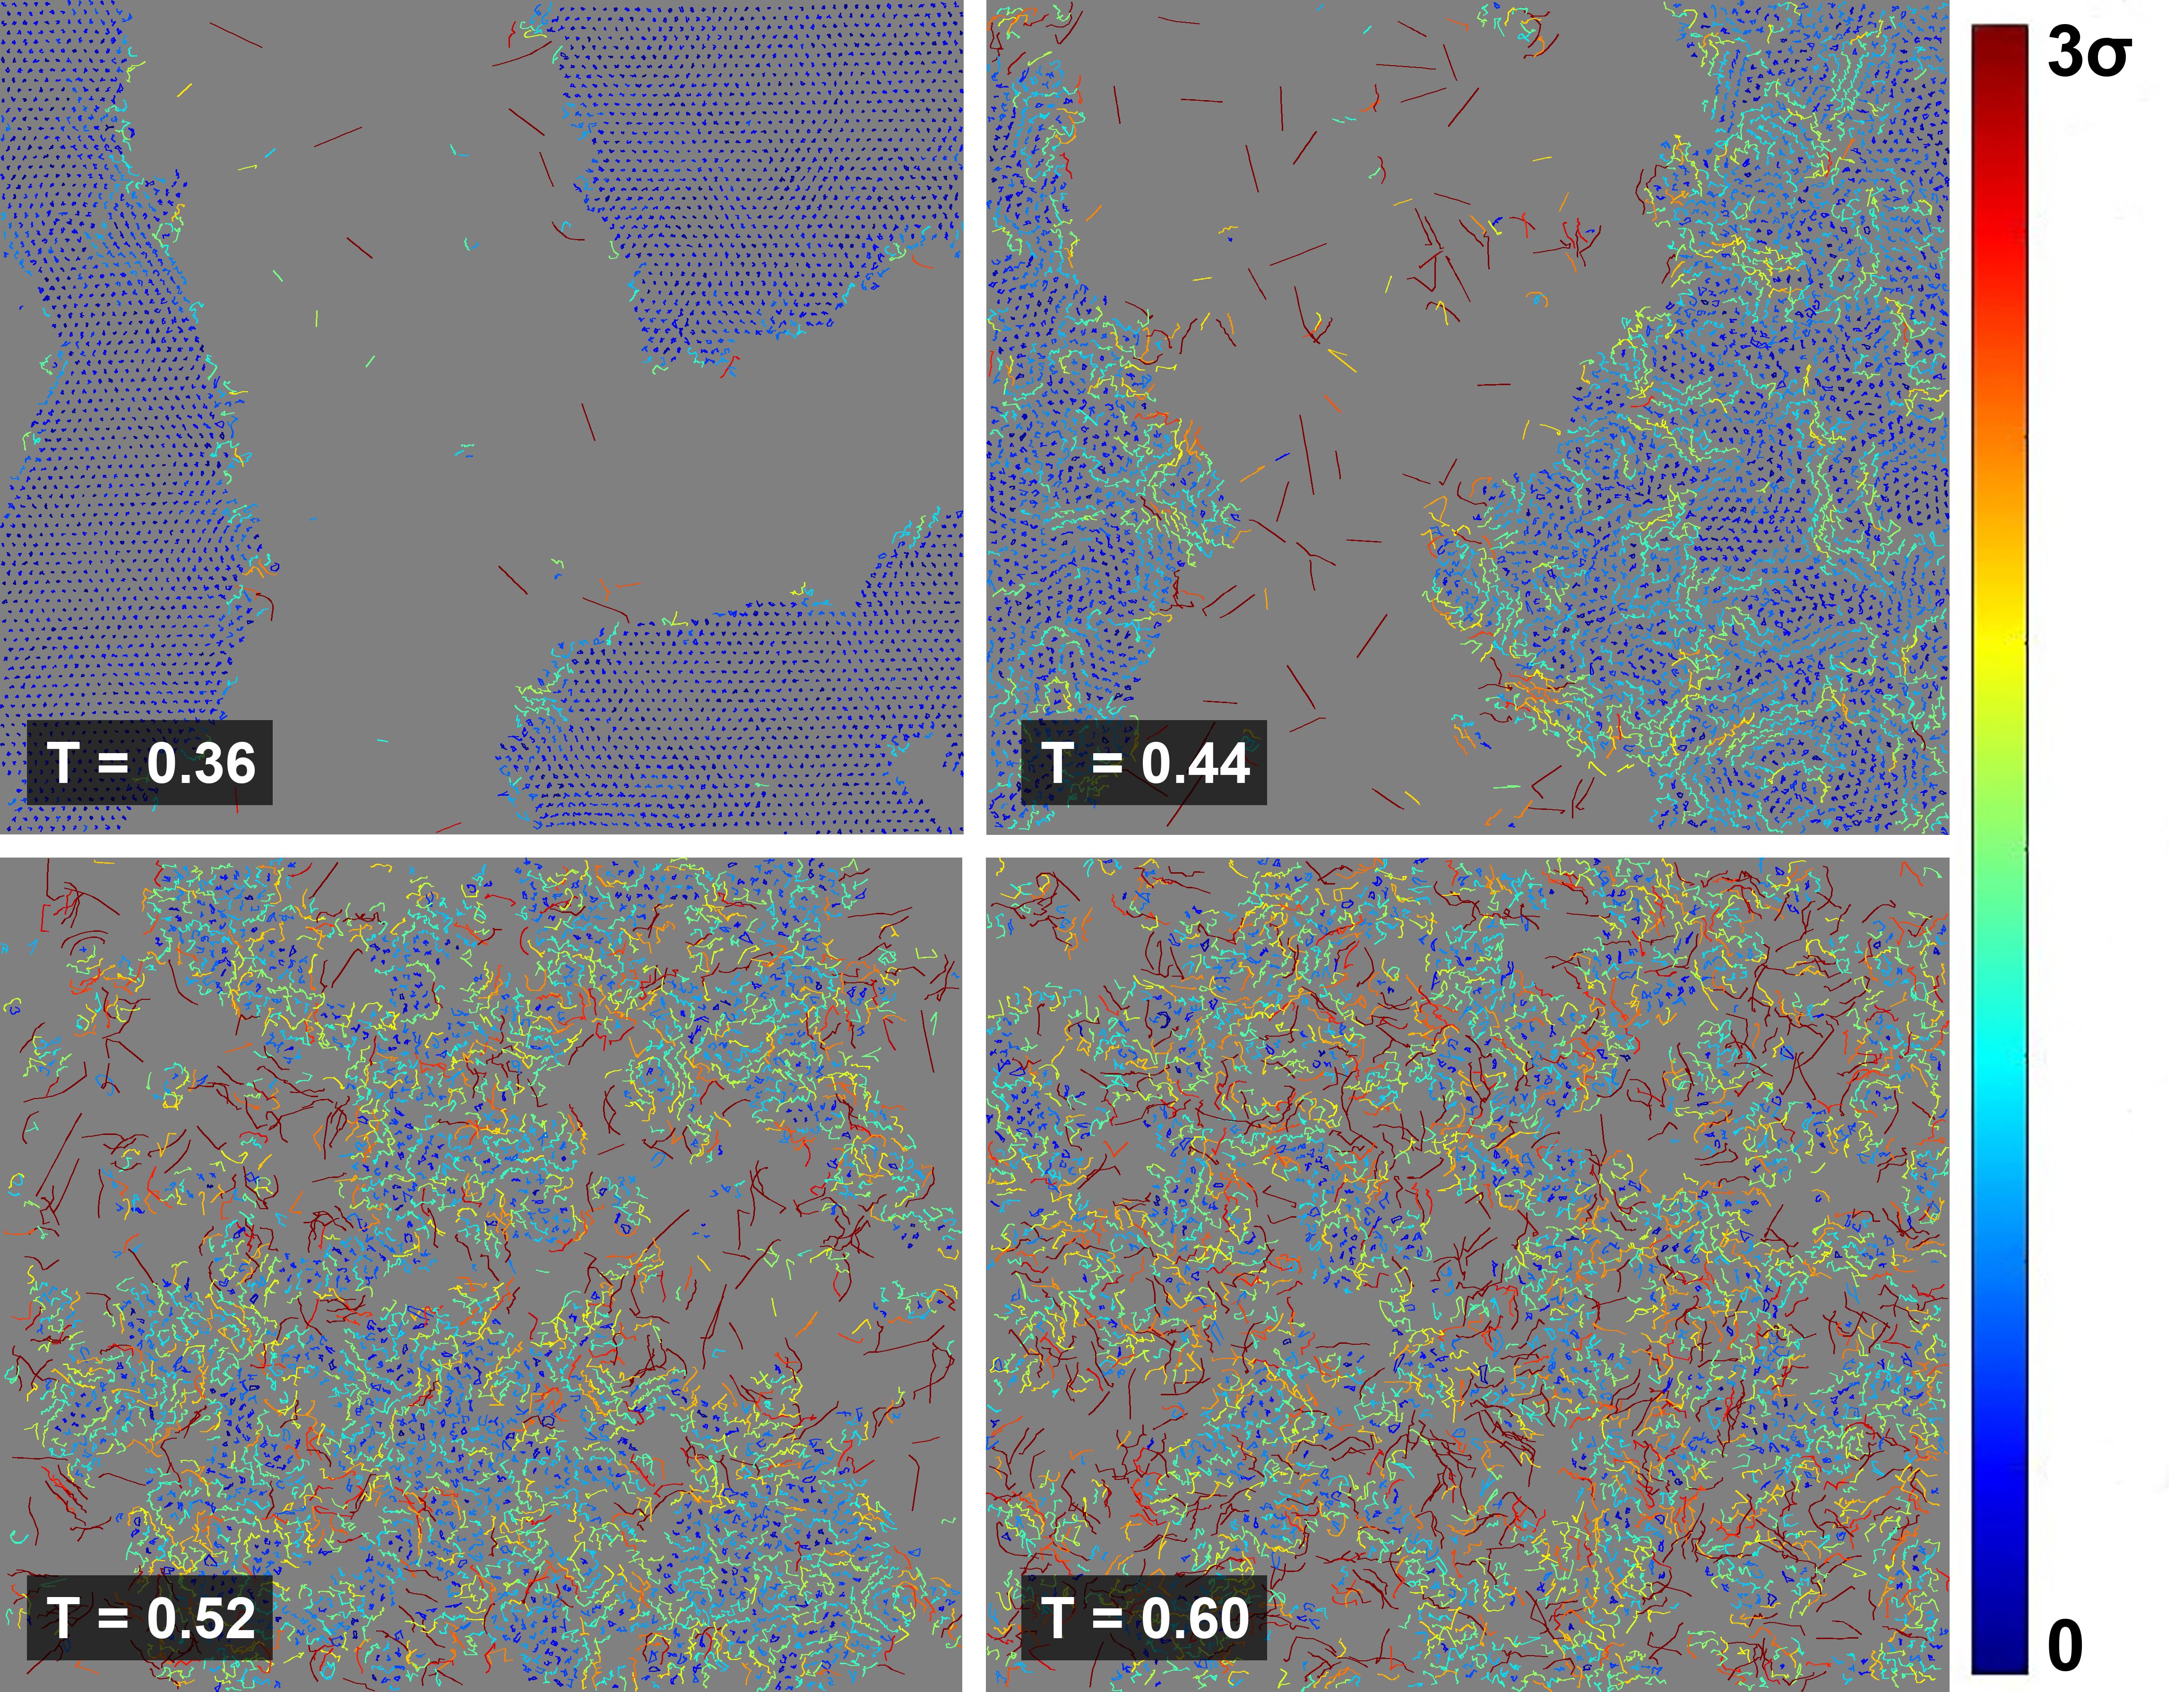
\includegraphics[width=0.7\textwidth]{Diffusion}
\caption{Смещение частиц от начального положения за 10 кадров моделирования. Цветом показана величина смещения в $\sigma$ (единица измерения длинны). Наиболее подвижным частицам соответствует темно-красный цвет траектории.}
\label{risTreck}
\end{center}
\end{figure}

Количество частиц на кадре в общем случае может быть не одинаковым. В реальных экспериментах с коллоидными суспензиями это обусловлено смещением частиц за пределы кадра, или потерей частицы на кадре из-за неидеальности распознавания объектов на изображении используемым методом. В случае моделирования причинами непостоянства количества частиц могут быть смещение частицы за пределы исследуемой области, либо отсева частиц с бесконечными гранями ячейки вороного, расположенной на периферии, для которой не удается определить не соседей, ни площади. Такие частицы не участвуют в статистике ни расчета термодинамических параметров во второй главе, ни в расчете параметров переноса. 

Зная смещения всех частиц от их изначального положения в системе, с $t = 0$, можно рассчитать среднеквадратичное смещение частиц с помощью уравнения:
\begin{equation}
    \sigma^2(t) = \sum\limits_{\alpha = 1}^{N(t)} (r_{\alpha}(t) - r_{\alpha}(0))^2 / N(t),
    \label{eqRMS}
\end{equation}
где $\sigma^2(t)$ - среднеквадратичное смещение частиц, $N(t)$ - количество частиц в данный момент времени в кадре, $r_{\alpha}(t)$ - положение частицы в момент времени $t$, $r_{\alpha}(0)$ - положение частицы в начальный момент времени $t = 0$.

\begin{figure}[h]
\begin{center}
\begin{minipage}[h]{0.45\linewidth}
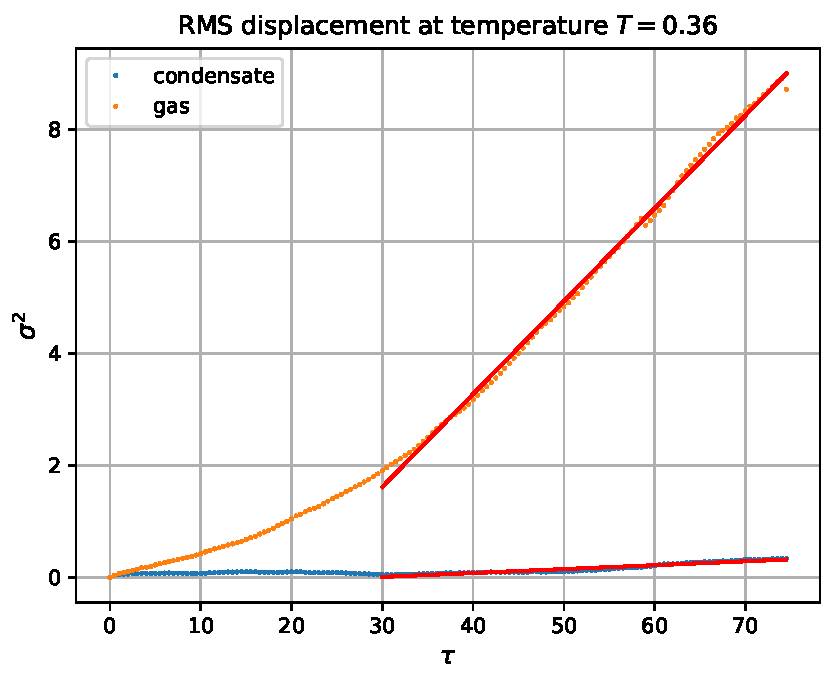
\includegraphics[width=\textwidth, keepaspectratio]{diffusion_fit_0.36}
\end{minipage}
%\hfill
\begin{minipage}[h]{0.45\linewidth}
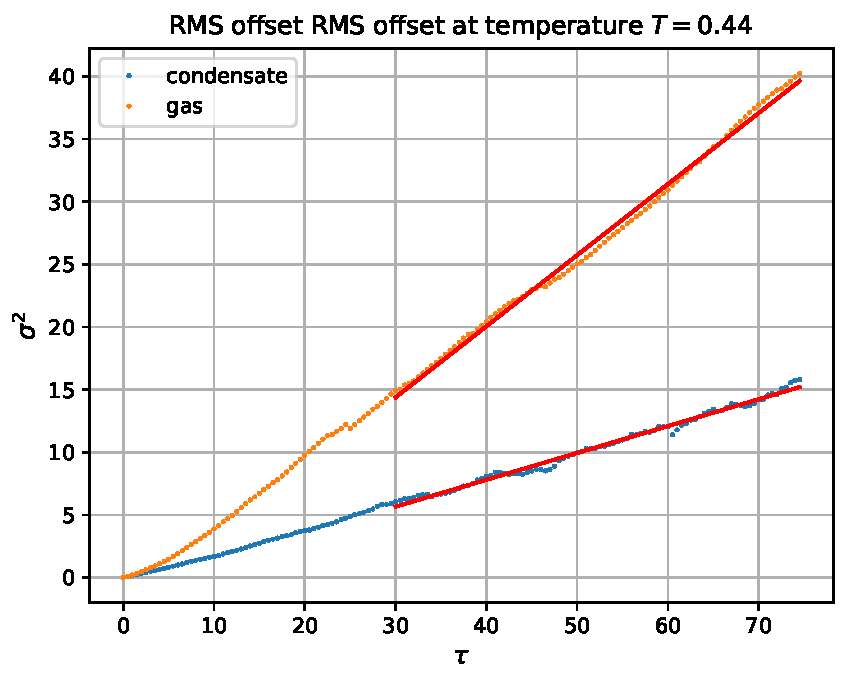
\includegraphics[width=\textwidth, keepaspectratio]{diffusion_fit_0.44}
\end{minipage}

\begin{minipage}[h]{0.45\linewidth}
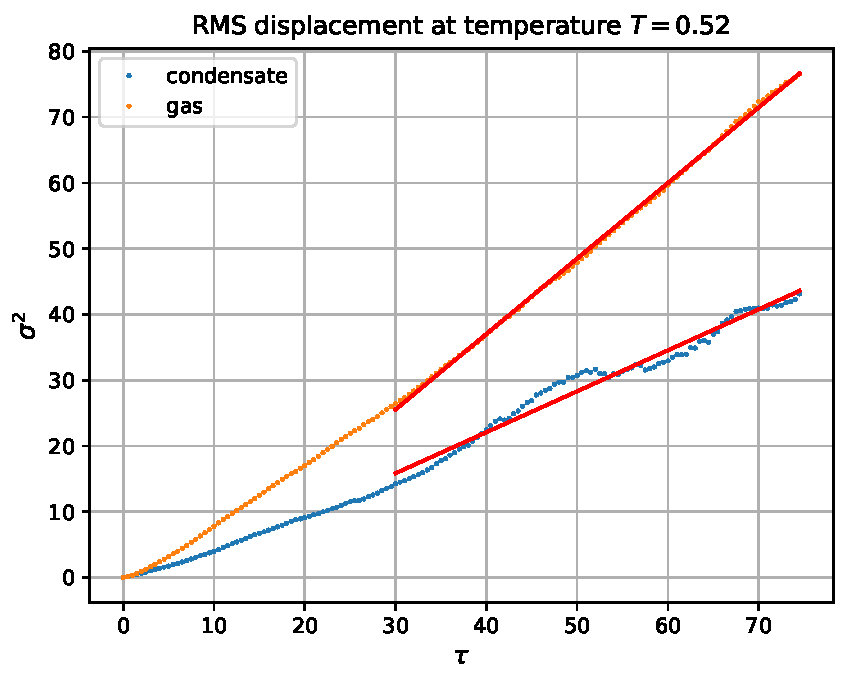
\includegraphics[width=\textwidth, keepaspectratio]{diffusion_fit_0.52}
\end{minipage}
%\hfill
\begin{minipage}[h]{0.45\linewidth}
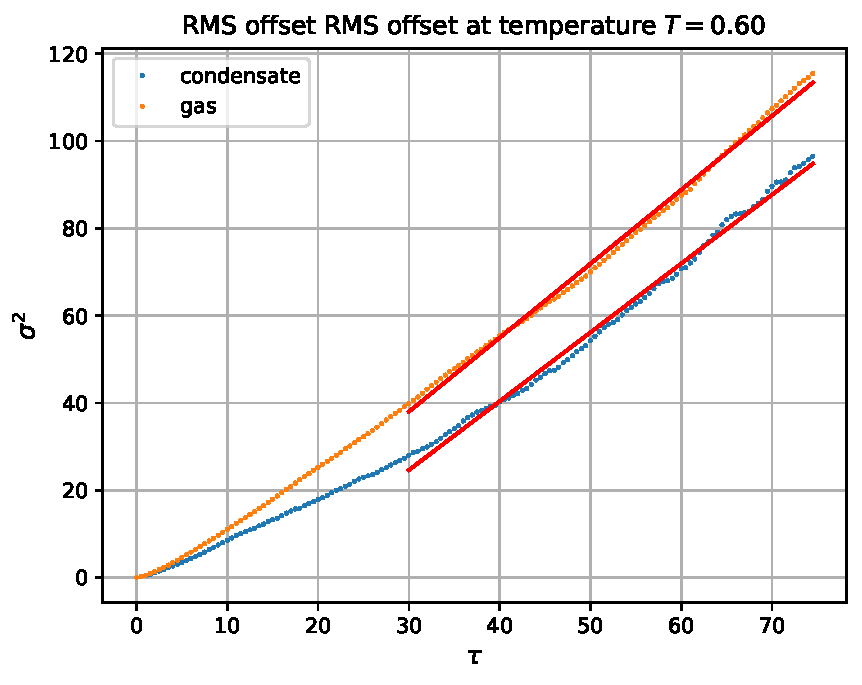
\includegraphics[width=\textwidth, keepaspectratio]{diffusion_fit_0.60}
\end{minipage}
\caption{Временная зависимость среднеквадратичного смещения частиц для различных температур на примере потенциала Леннарда-Джонса. Синим цветом обозначено среднеквадратичное смещение конденсированных частиц,  а оранжевым - всех частиц в исследуемой системе.}
\label{risRMS}
\end{center}
\end{figure}

График зависимости среднеквадратичного смещения для подсистем конденсированных частиц и всех (все частицы в системе, включая газовые и конденсат) от безразмерного времени для различных температур изображен на рисунке \ref{risRMS}.

Так как для двумерной системы верно равенство $\sigma^2(t) = 4Dt$, то коэффициент диффузии выражается следующей формулой:
\begin{equation}
    D = \frac{\sigma^2(t)}{4t},
    \label{eqD}
\end{equation}
где $D$ - коэффициент диффузии в веществе.

Его можно получить путем аппроксимации среднеквадратичного смещения функцией $\sigma^2(t) = 4Dt + a$, где $a$ - подгоночный коэффициент. Подгоночный коэффициент $a$ появляется в следствие того, что аппроксимация производится начиная не с 0 по времени, а с некоторого значения, когда функция становится линейной. Данный эффект хорошо наблюдается при $T = 0.36$ на рисунке \ref{risRMS}. экспериментально установлено, что для данных экспериментов достаточно использовать последние $60\%$ точек, для правильной аппроксимации. 
На рисунке \ref{risRMS} она показана сплошной красной линией, которая аппроксимирует среднеквадратичное смещение с достаточно хорошей точностью.

\begin{figure}[h]
\begin{center}
\begin{minipage}[h]{0.45\linewidth}
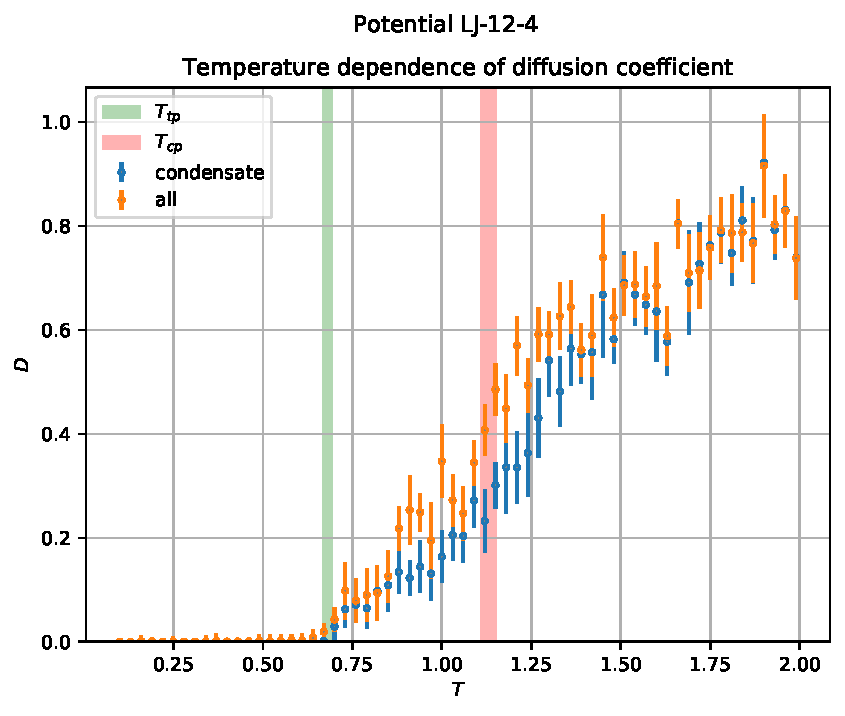
\includegraphics[width=\textwidth, keepaspectratio]{plot_diffusion_Potential LJ-12-4_1}
\end{minipage}
\begin{minipage}[h]{0.45\linewidth}
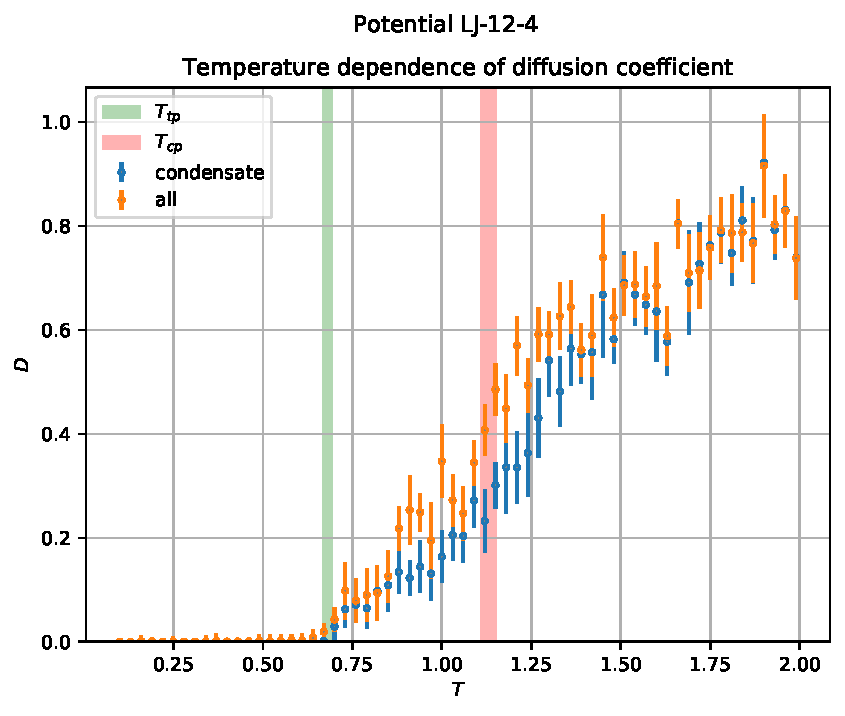
\includegraphics[width=\textwidth, keepaspectratio]{plot_diffusion_Potential LJ-12-4_1}
\end{minipage}
\begin{minipage}[h]{0.45\linewidth}
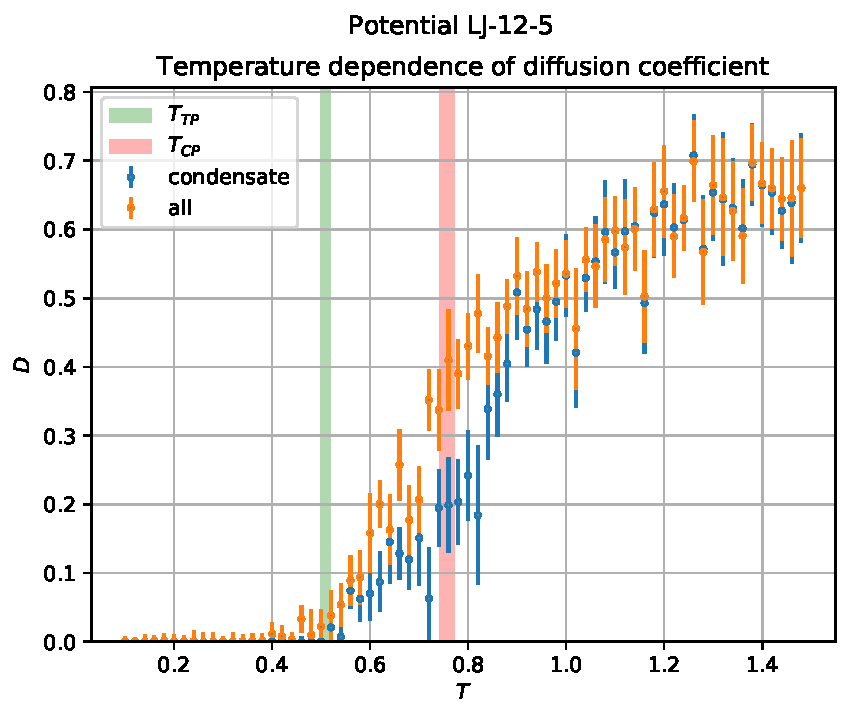
\includegraphics[width=\textwidth, keepaspectratio]{plot_diffusion_Potential LJ-12-5_1}
\end{minipage}
\begin{minipage}[h]{0.45\linewidth}
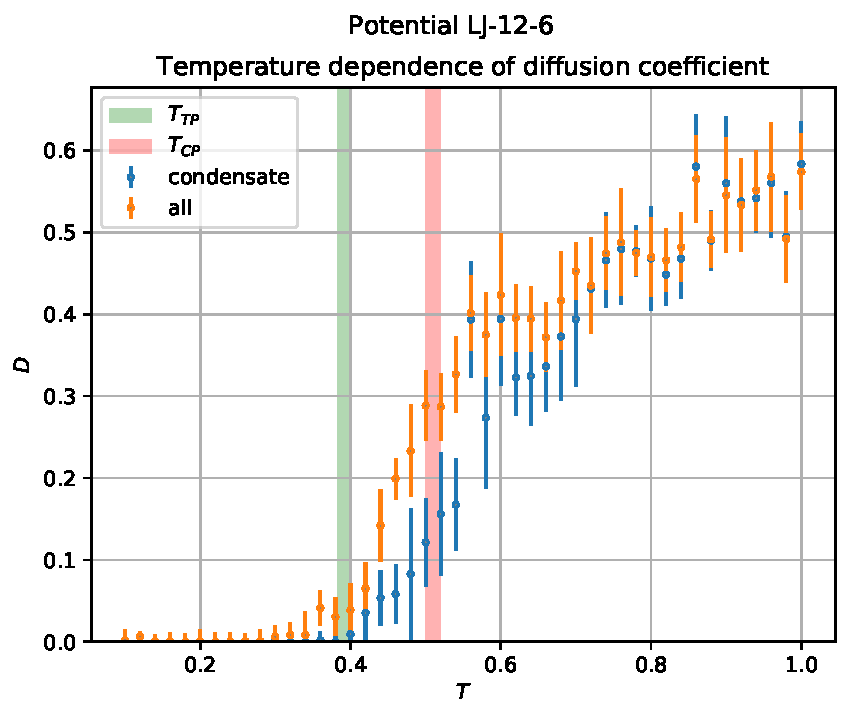
\includegraphics[width=\textwidth, keepaspectratio]{plot_diffusion_Potential LJ-12-6_1}
\end{minipage}
\caption{Температурная зависимость коэффициента диффузии для различных потенциалов взаимодействия. Не доделана!}
\label{risD}
\end{center}
\end{figure}

Проводя данные вычисления для различных температур, можно установить температурную зависимость коэффициента диффузии для различных потенциалов взаимодействия, изображенную на рисунке \ref{risD}.

Полученные результаты хорошо согласуются с экспериментом, например в $LJ12-6$ температура плавления $T_{TP} = 0.405$, что соответствует температуре, при которой значение коэффициента диффузии начинает расти.

Коэффициент диффузии, рассчитанный таким образом, может быть использован для определения тройной точки, так как однозначно при различных потенциалах показывает резкий рост смещения частиц относительно своих изначальных положений, что характерно при плавлении веществ.

\begin{figure}[h]
\begin{center}
\begin{minipage}[h]{0.45\linewidth}
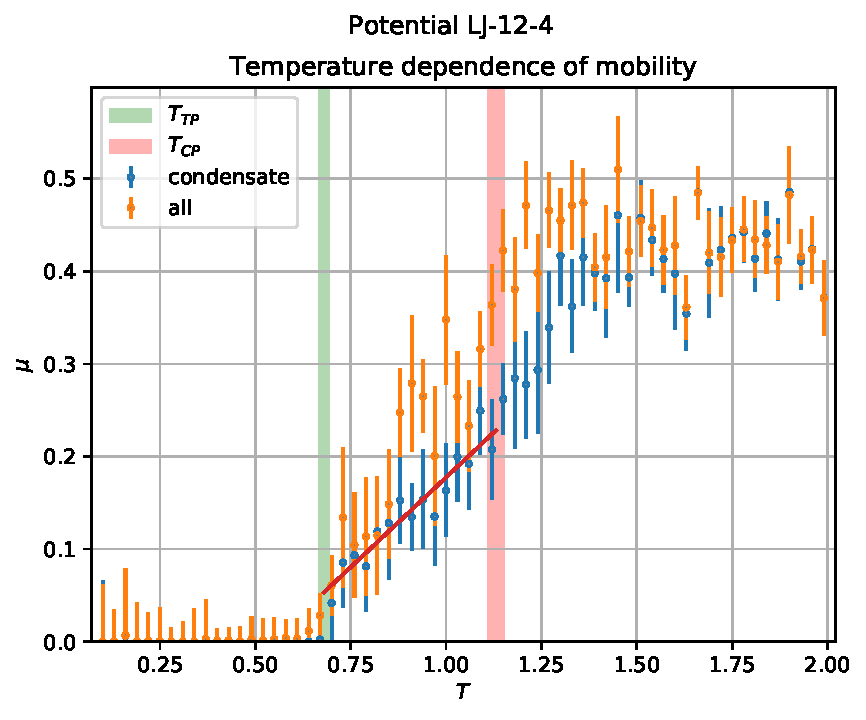
\includegraphics[width=\textwidth, keepaspectratio]{plot_mobility_Potential LJ-12-4_1}
\end{minipage}
%\hfill
\begin{minipage}[h]{0.45\linewidth}
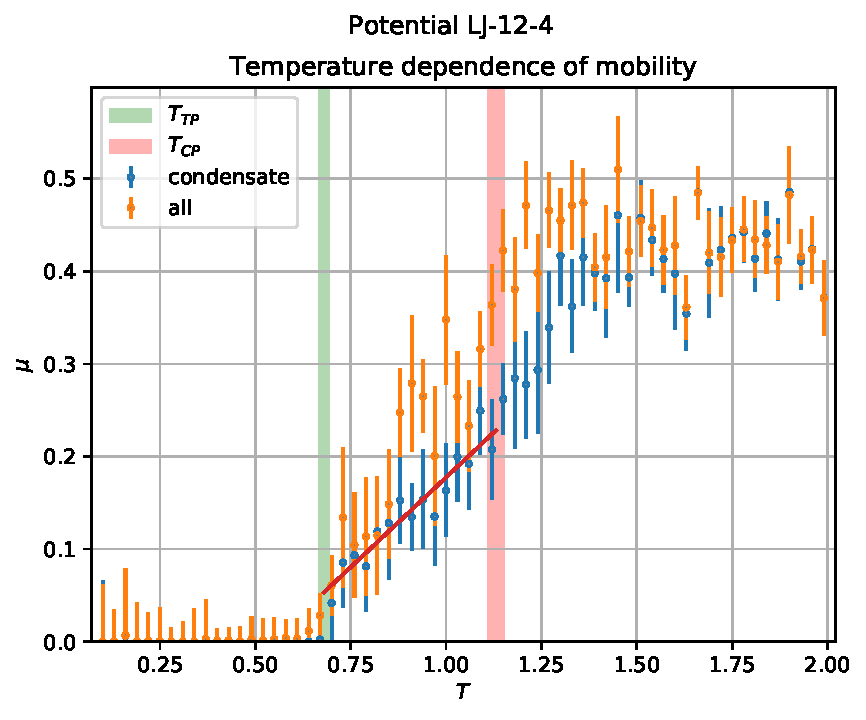
\includegraphics[width=\textwidth, keepaspectratio]{plot_mobility_Potential LJ-12-4_1}
\end{minipage}
\begin{minipage}[h]{0.45\linewidth}
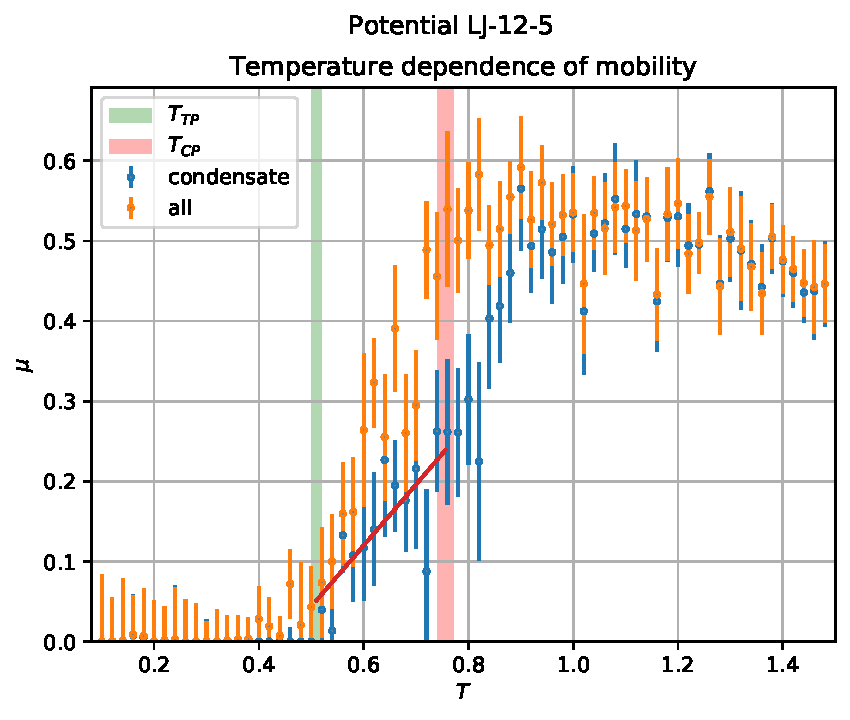
\includegraphics[width=\textwidth, keepaspectratio]{plot_mobility_Potential LJ-12-5_1}
\end{minipage}
%\hfill
\begin{minipage}[h]{0.45\linewidth}
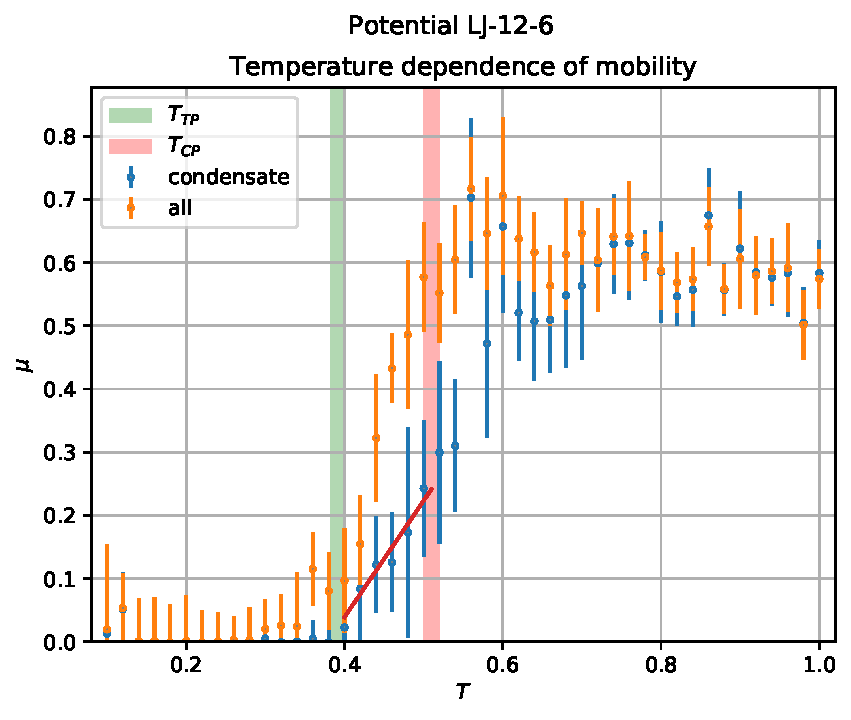
\includegraphics[width=\textwidth, keepaspectratio]{plot_mobility_Potential LJ-12-6_1}
\end{minipage}
\caption{Температурная зависимость мобильности для различных потенциалов взаимодействия. Не доделана!}
\label{risMuDiff}
\end{center}
\end{figure}

Кроме диффузии мы можем вычислить мобильность частиц в системе, которая определяется следующим образом:
\begin{equation}
    \mu  = \frac{D}{T},
    \label{eqMuDiff}
\end{equation}
где $\mu$ - мобильность частиц.

Зависимость мобильности частиц от температуры представлена на рисунке \ref{risMuDiff}.
Как можно заметить, данная зависимость скорее всего линейна в промежутке от тройной до критической точки, что требует дальнейшего теоретического обоснования.

\section{Связь термодинамических параметров и параметров переноса вещества}\label{C3_2}

В попытках выяснить зависимость параметров переноса вещества от его термодинамических параметров, были построены зависимости мобильности от сжимаемости и диффузии (рисунки \ref{risMuBeta}, \ref{risDBeta}), а так же зависимость скорости звука от мобильности (рисунок \ref{risCMu}).

\begin{figure}[h]
\begin{center}
\begin{minipage}[h]{0.45\linewidth}
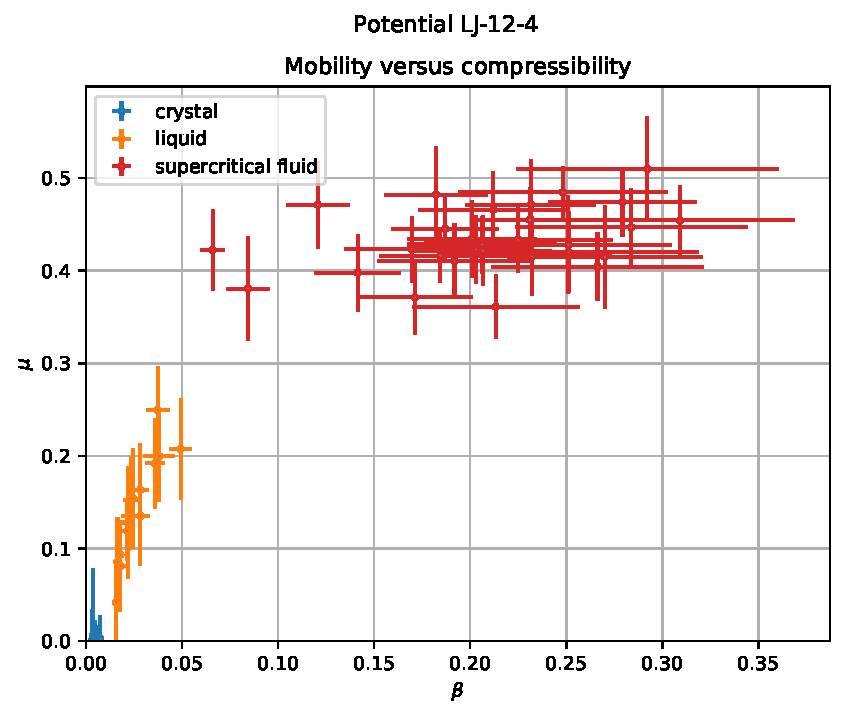
\includegraphics[width=\textwidth, keepaspectratio]{plot_compress_mobility_Potential LJ-12-4_1}
\end{minipage}
%\hfill
\begin{minipage}[h]{0.45\linewidth}
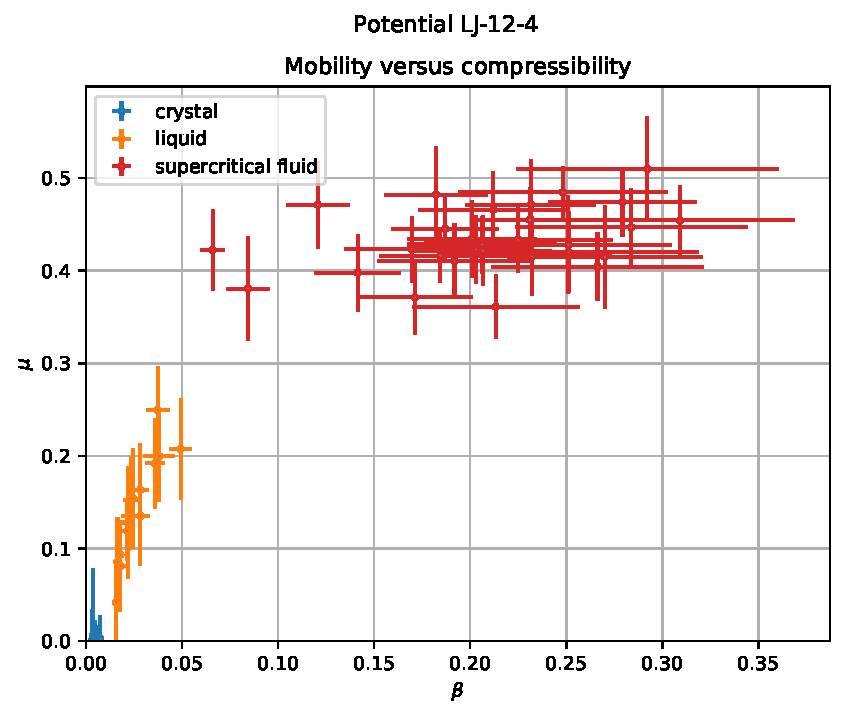
\includegraphics[width=\textwidth, keepaspectratio]{plot_compress_mobility_Potential LJ-12-4_1}
\end{minipage}

\begin{minipage}[h]{0.45\linewidth}
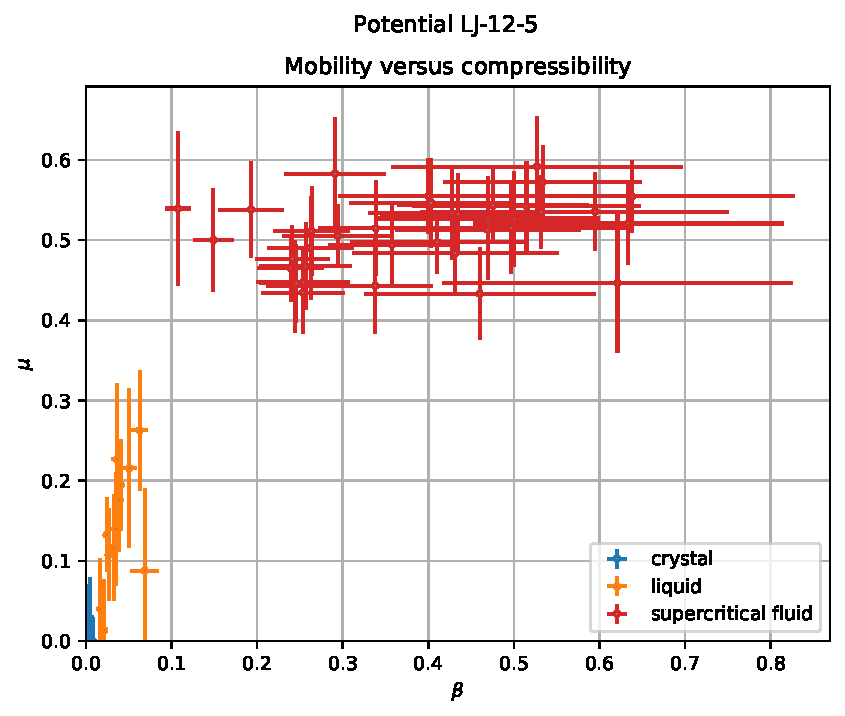
\includegraphics[width=\textwidth, keepaspectratio]{plot_compress_mobility_Potential LJ-12-5_1}
\end{minipage}
%\hfill
\begin{minipage}[h]{0.45\linewidth}
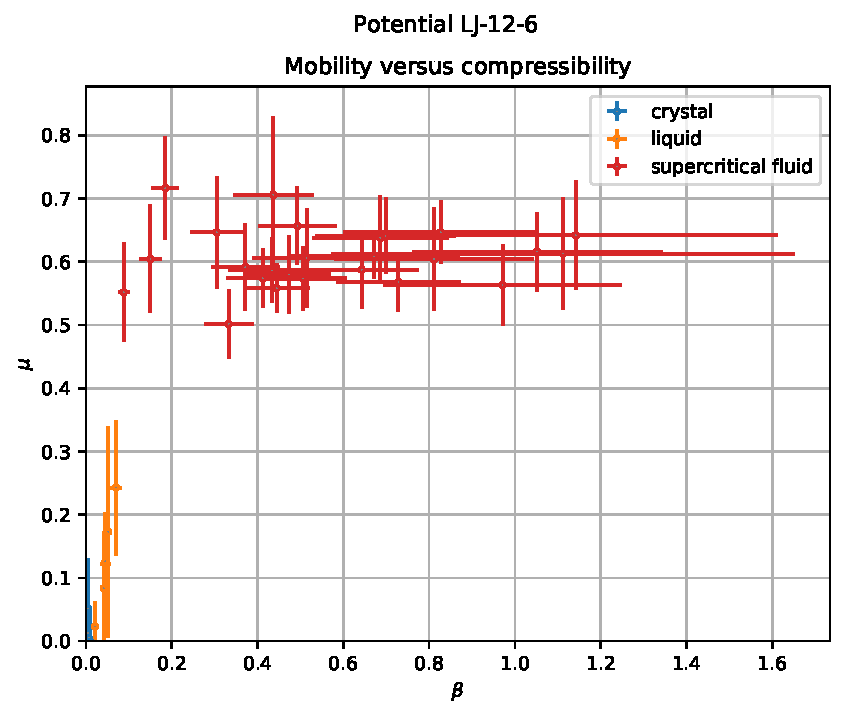
\includegraphics[width=\textwidth, keepaspectratio]{plot_compress_mobility_Potential LJ-12-6_1}
\end{minipage}
\caption{Зависимость мобильности от сжимаемости. Не доделана!}
\label{risMuBeta}
\end{center}
\end{figure}


\begin{figure}[h]
\begin{center}
\begin{minipage}[h]{0.45\linewidth}
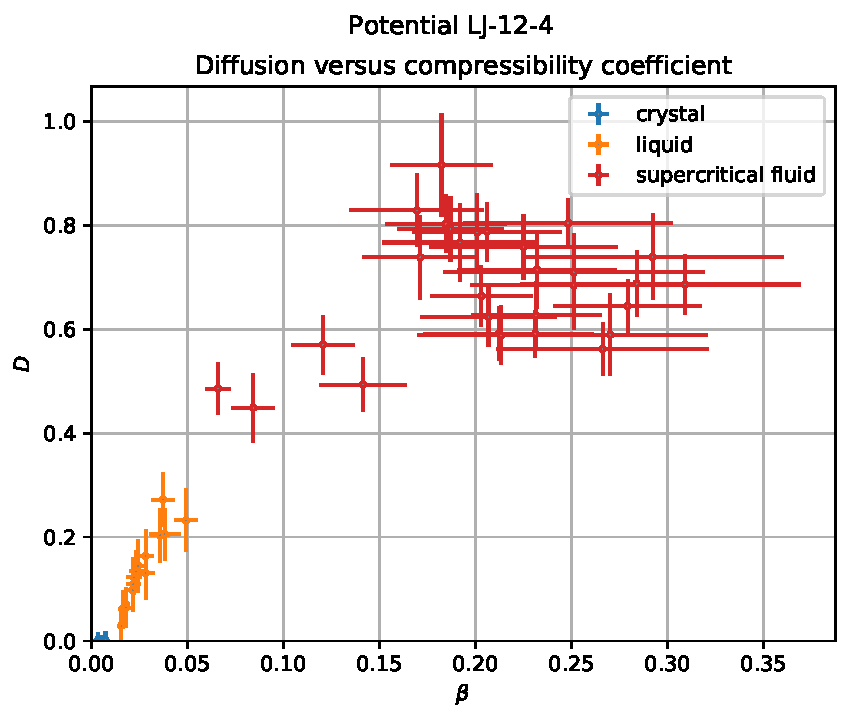
\includegraphics[width=\textwidth, keepaspectratio]{plot_diffusion_compress_Potential LJ-12-4_1}
\end{minipage}
%\hfill
\begin{minipage}[h]{0.45\linewidth}
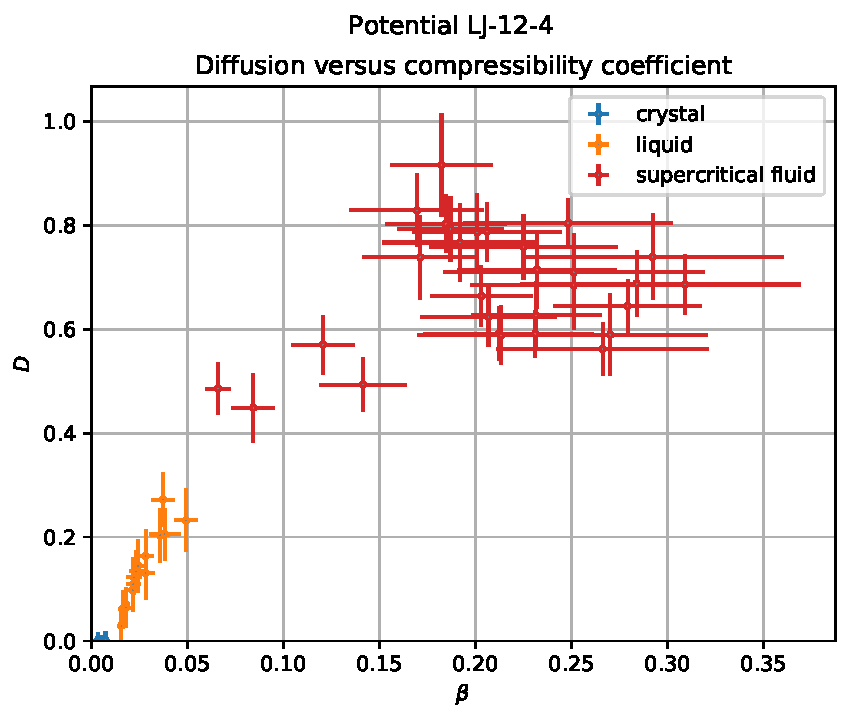
\includegraphics[width=\textwidth, keepaspectratio]{plot_diffusion_compress_Potential LJ-12-4_1}
\end{minipage}

\begin{minipage}[h]{0.45\linewidth}
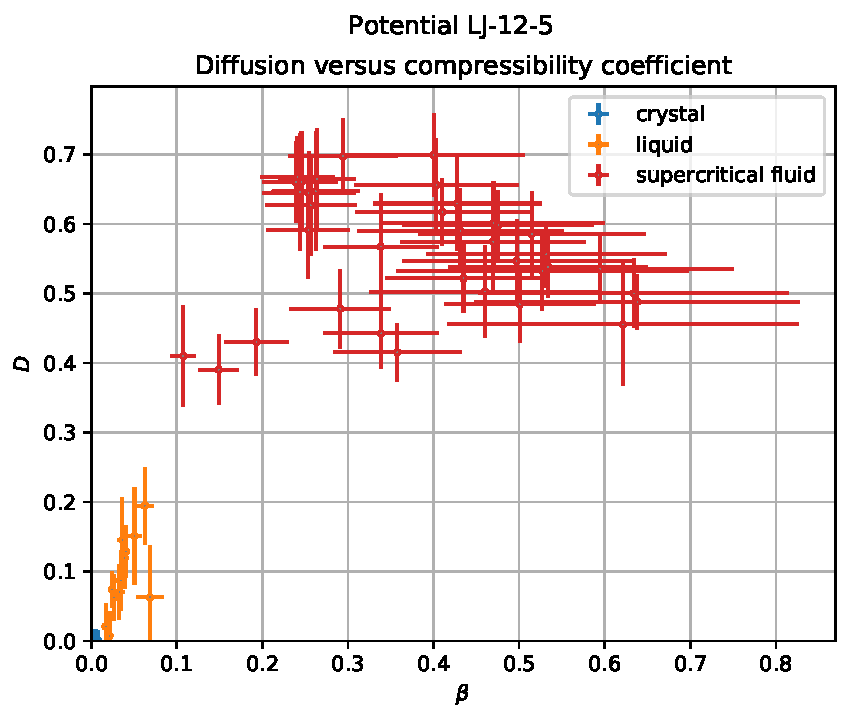
\includegraphics[width=\textwidth, keepaspectratio]{plot_diffusion_compress_Potential LJ-12-5_1}
\end{minipage}
%\hfill
\begin{minipage}[h]{0.45\linewidth}
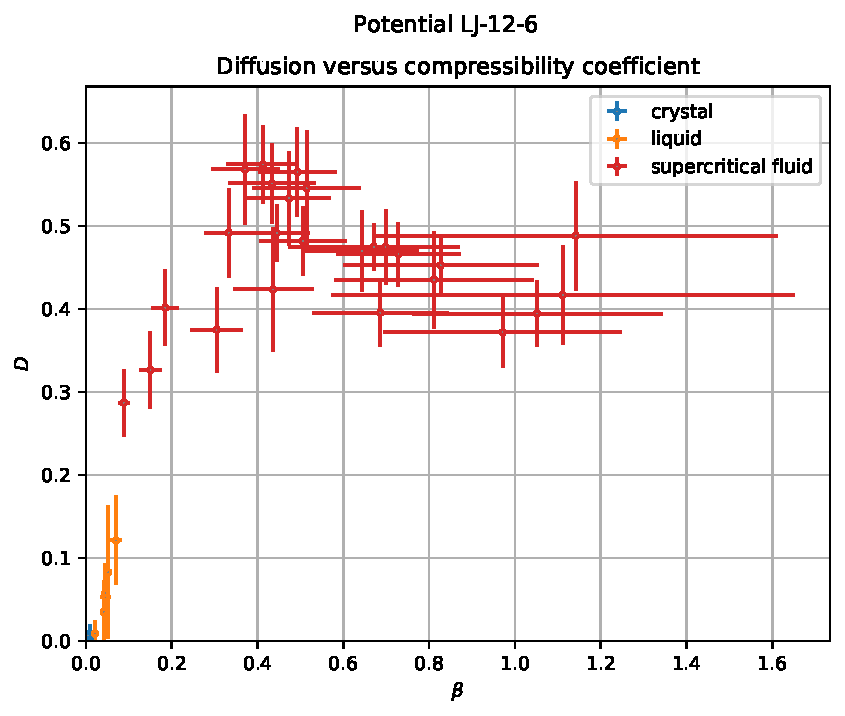
\includegraphics[width=\textwidth, keepaspectratio]{plot_diffusion_compress_Potential LJ-12-6_1}
\end{minipage}
\caption{Зависимость диффузии от сжимаемости. Не доделана!}
\label{risDBeta}
\end{center}
\end{figure}



\begin{figure}[h]
\begin{center}
\begin{minipage}[h]{0.45\linewidth}
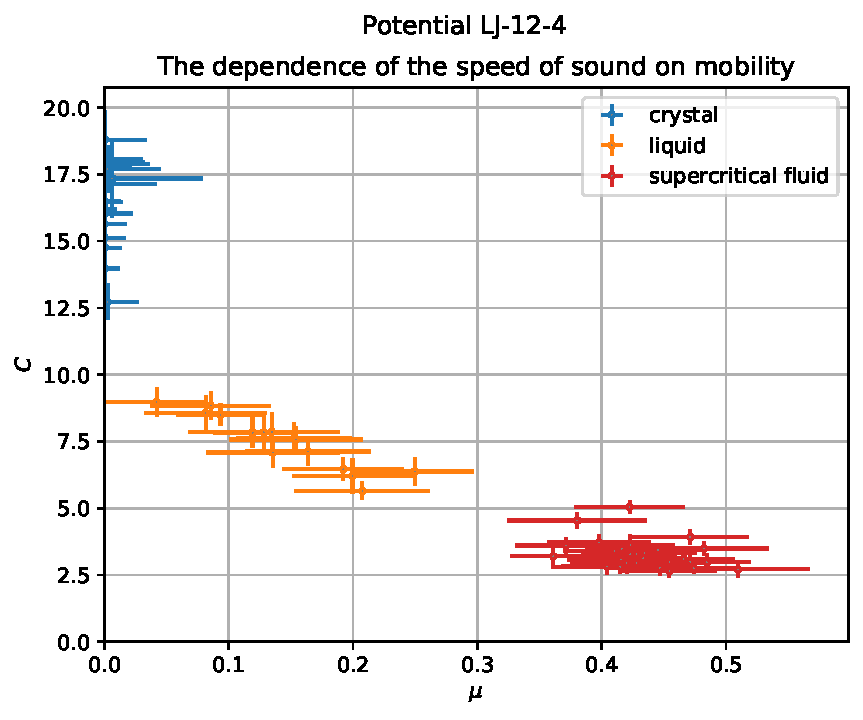
\includegraphics[width=\textwidth, keepaspectratio]{sound_speed_mobility_Potential LJ-12-4_1}
\end{minipage}
%\hfill
\begin{minipage}[h]{0.45\linewidth}
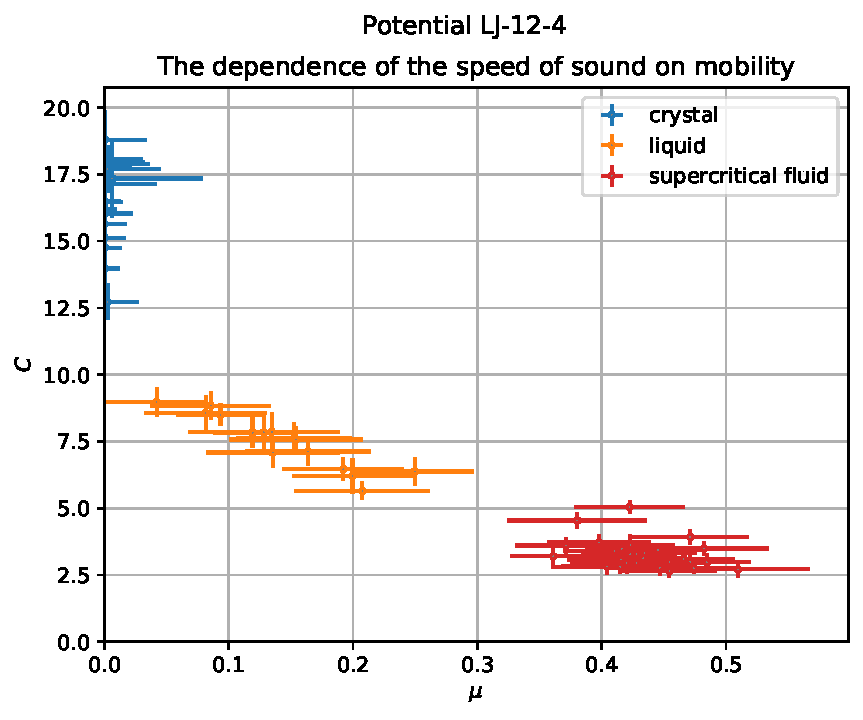
\includegraphics[width=\textwidth, keepaspectratio]{sound_speed_mobility_Potential LJ-12-4_1}
\end{minipage}

\begin{minipage}[h]{0.45\linewidth}
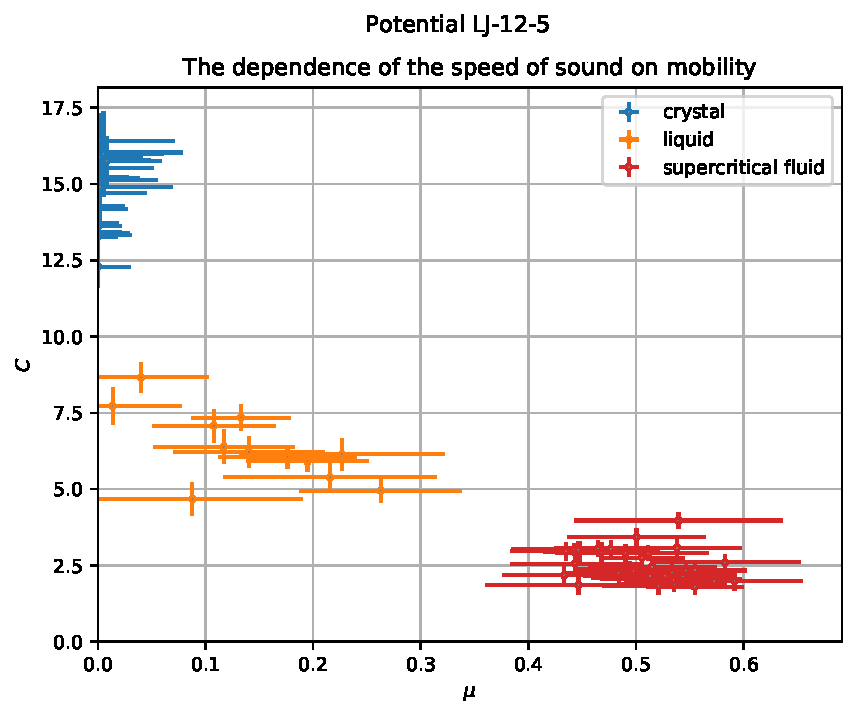
\includegraphics[width=\textwidth, keepaspectratio]{sound_speed_mobility_Potential LJ-12-5_1}
\end{minipage}
%\hfill
\begin{minipage}[h]{0.45\linewidth}
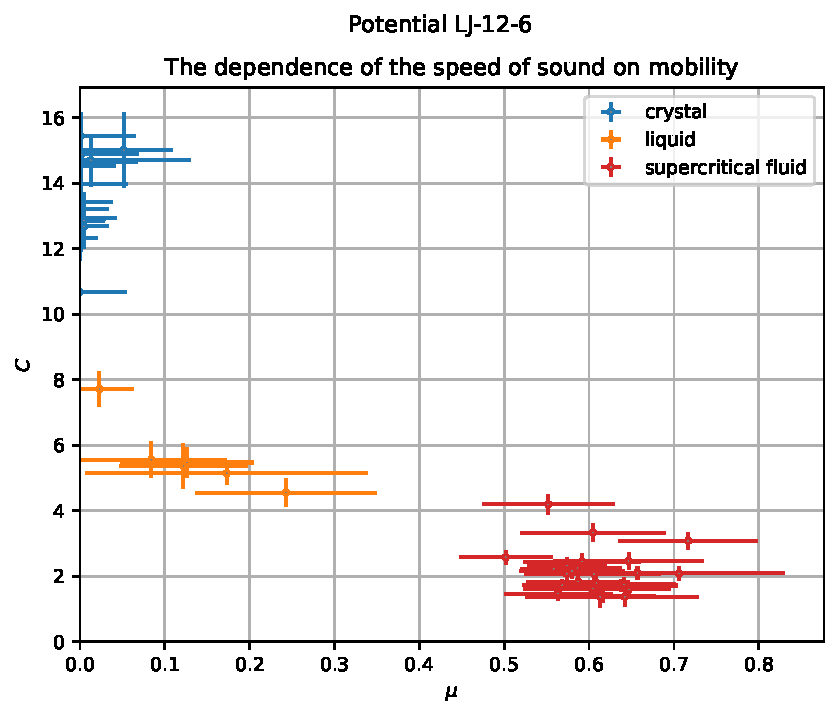
\includegraphics[width=\textwidth, keepaspectratio]{sound_speed_mobility_Potential LJ-12-6_1}
\end{minipage}
\caption{Зависимость скорости звука от мобильности. Не доделана!}
\label{risCMu}
\end{center}
\end{figure}

Скорее всего данные зависимости описываются корневой функцией.


\section{Выводы главы}\label{C3_3}

В данной главе были рассмотрены расчеты диффузии методами молекулярной динамики, и его особенности. Данный метод, в совокупности с методом распознавания фаз, описанном в разделе \ref{C2_1}, позволяет с высокой точностью определить температуру плавления веществ, независимо от потенциала взаимодействия.

Так же было установлено, что зависимость мобильности частиц от тройной до критической точки имеет линейную зависимость.
